\chapter{Konzeption der Anwendung}\label{chapter_3}
Im vorigen Kapitel wurden die Anforderungen, sowie das Umfeld der Arbeit erläutert. In diesem Abschnitt wird der aktuelle Workflow beim Konfigurieren analysiert und anschließend an die mobile Umgebung angepasst. Nach der Workflow-Modellierung wird mit einer Entscheidung über den richtigen Typ der App.

\section{Aktueller Konfigurationsprozess}
Im aktuellen Prozess des Kunden wird ein Upgrade zuerst über den Produktkatalog gefunden. Im Katalog ist eine eindeutige Nummer enthalten, die bei der Bestellung verwendet wird. Die Fluggesellschaft nennt zu der Upgrade-Nummer, die Flugzeuge, die dieses Upgrade erhalten sollen. Diese Informationen werden von einem Design-Manager angenommen. Für die Weiterverarbeitung werden diese Informationen im Konfigurator-Client aus Abschnitt \ref{airbusConfigurator} erfasst. Die einzelnen Schritte der Erfassung sind in Abbildung \ref{webguiWorkflow} zu sehen. \par
\begin{figure}
\label{webguiWorkflow}
\centering
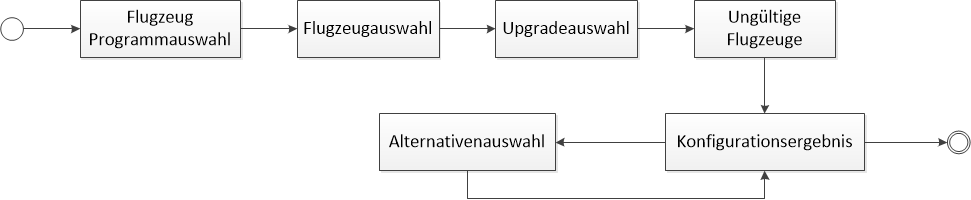
\includegraphics[width=300px]{images/workflow_webgui}
\caption{Programmablauf des Konfigurations-Clients}
\end{figure}
Im ersten Schritt wird das passende Flugzeugprogramm ausgewählt. Ein Programm ist eine grobe Einteilung für Flugzeuge nach deren Größe und Art. Die Auswahl ist eine erste Filterung der Datensätze. Des weiteren wird mit Hilfe des Programms das Regelwerk, welches auf dem Konfigurationsserver verwendet wird festgelegt. Anschließend folgt die Auswahl der entsprechenden Flugzeuge, welche ein Upgrade erhalten sollen. Die Auswahl kann nach bestimmten Kriterien gefiltert werden. Bei der Bestellung eines Upgrades wird die Flugzeugnummer angegeben, womit eine schnelle Auswahl erfolgen kann. Sind die Flugzeuge ausgewählt, werden Upgrades aus einer Liste selektiert. Es sind alle verfügbaren Updates aufgelistet. Die Auswahl erfolgt ebenfalls mit der eindeutigen Nummer, welche bei der Bestellung angegeben wurde. \par 

Nach der letzten Auswahl sind alle für die Konfiguration benötigten Elemente ausgewählt. Es folgt eine Validierung der Flugzeuge. Bei dieser Überprüfung werden die einzelnen Flugzeuge auf Konfigurationen untersucht, die in Widerspruch mit dem ausgewählten Upgrade stehen. Wenn keine Widersprüche gefunden wurden, ist die Bildung von sogenannten Konfigurationsgruppen die nächste Aufgabe. Eine Konfigurationsgruppe enthält Flugzeuge, die in die gleichen Zielzustände kommen, wenn das Upgrade eingebaut wird. Wenn es mehrere Möglichkeiten gibt, um in einen bestimmten Zustand des Flugzeuges zu kommen, werden sogenannte Alternativen in einer Konfigurationsgruppe enthalten. Damit die Konfiguration vollständig ist, muss der Anwender für die Gruppe eine Alternative auswählen. \par

Nachdem eine vollständige Konfiguration erzeugt wurde, wird daraus ein Excel-Dokument generiert. In diesem sind die Upgrades enthalten, die in den einzelnen Flugzeuge eingebaut werden müssen. Aus dem Dokument wird ein Upgrade-Angebot erstellt, dass anschließend dem Kunden vorgelegt wird.

\section{Workflow Modellierung}
Beim derzeitigen Konfigurationsprozess wird die eigentliche Konfiguration dem Experten überlassen. Ein Kunde wählt die Codes und Identifikationsnummern aus Katalog und derzeitigem Flugzeugbestand aus, erhält jedoch erst nach der Arbeit des Experten eine Bestätigung über die Gültigkeit der Konfiguration. Dieser Prozess wird bei der Portierung auf die mobile Umgebung verändert, so dass ein neuer Workflow entsteht. Die Prozesse sind im Folgenden in einen mobilen Konfigurationsprozess und den unterstützenden App-Workflow unterteilt.
\subsection{Mobiler Konfigurationsprozess}
Der derzeitige Workflow sollte die neuen Möglichkeiten einer mobilen Konfigurationsumgebung beinhalten. Mit der Mobilität ist ein Szenario einer direkten Konfiguration mit dem Kunden und einem Vertriebsexperten möglich. Beide können mithilfe der App direkt kommunizieren und das Ugrade gemeinsam durchführen. 
Primäres Ziel dieser Anpassung ist den Prozess kundenfreundlicher zu gestalten. Dieses Ziel soll durch folgende zwei Maßnahmen erreicht werden: \par

\begin{itemize}
        \item \textbf{Vereinfachung der Auswahl:} Das An- und Abwählen der Flugzeuge, bzw. der Upgrades soll vereinfacht werden. Die Auswahl soll nicht nur durch die Produktcodes, sondern durch verständlichere Weise erfolgen. 
        \item \textbf{Schnelleres Feedback:} Durch eine mobile Lösung soll bereits beim Kunden ein Feedback über die Gültigkeit der Konfiguration vorhanden sein.
\end{itemize}

Mit beiden Maßnahmen wird der Kunde stärker in den Prozess der Konfiguration einbezogen. Im Idealfall kann der Kunde die Anwendung alleine bedienen und der Experte steht nur Beratend zur Seite. Eine weitere Besonderheit der neuen Anwendung kann sein, dass der Kunde zu einem weiteren Upgrade bewogen wird, welches er erst beim Benutzen der Anwendung entdeckt. Eine weitere Möglichkeit ist das gezielte Anzeigen von kundenspezifische Informationen, die für weitere Kaufaktivitäten sorgen können. \par

\subsection{Workflow der App}
Der Anwendungsworkflow muss zu dem neuen fachlichen Prozess passen und ihn unterstützen. Dies geschieht durch Anpassungen an die Kommunikation mit dem Konfigurationsserver. 
Der aktuelle Client und der Server befinden sich auf der gleichen Umgebung. Somit können beide direkt miteinander kommunizieren und benötigen keine aufwändigen Webservice Schnittstellen. Für den neuen Prozess muss der Konfigurationsserver von der mobilen Umgebung erreichbar sein. Dies bedeutet, dass es eine Schnittstelle für die App geben muss. Die Kommunikation mit dem Webserver kann durch den mobilen Einsatz erschwert werden. Dies ist beispielsweise der Fall, wenn die Konfiguration beim Kunden vor Ort stattfindet und eine schlechte, bis gar keine Verbindung vorhanden ist. Aus diesem Grund ist bei den Nicht-Funktionalen Anforderung in Abschnitt \ref{non_functional_requirements} ein sogenannter Offline Modus enthalten, der die Zusammenstellung einer Konfiguration auch ohne Anbindung an den Konfigurator ermöglicht. Um eine flüssige Navigation gewährleisten zu können, muss die Kommunikation mit dem Server auf das Wesentliche konzentriert sein. Dies bedeutet, dass eine Konfiguration erst am Ende stattfindet und die einzelnen Schritte, die im derzeitigen Client durchgeführt werden zusammengelegt werden müssen. \par
\begin{figure}
\label{appWorkflow}
\centering
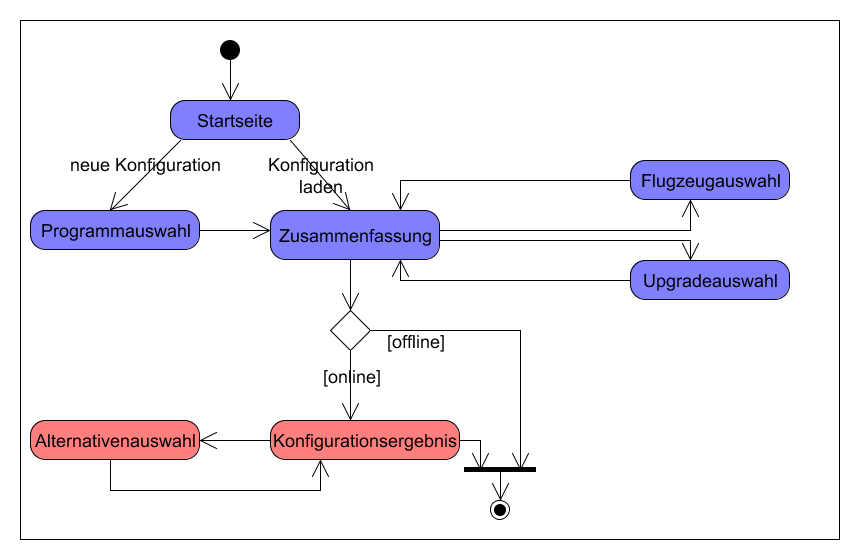
\includegraphics[width=400px]{images/workflow_app}
\caption{Programmablauf der Konfigurator-App}
\end{figure}
In Abbildung \ref{appWorkflow} ist der Anwendungsverlauf der App zu sehen. Analog zu der Weboberfläche wird bei einer neuen Konfiguration zuerst ein Programm (\textbf{Programmauswahl}) ausgewählt. Nach der Auswahl gelangt der Benutzer in eine \textbf{Zusammenfassung} der aktuellen Konfiguration. Von dieser Ansicht aus können Flugzeuge (\textbf{Flugzeugauswahl}) oder  Upgrades (\textbf{Upgradeauswahl}) selektiert werden. Sobald beides vorhanden ist, wird die Erreichbarkeit der Konfigurationsschnittstelle geprüft. Bei Verfügbarkeit befinden wir uns im "'Online"' Modus und es werden die Konfigurationsgruppen angezeigt. Nach erfolgter Konfiguration werden die Alternativen in einer separaten Ansicht (\textbf{Alternativenauswahl}) ausgewählt. Ist die Konfiguration vollständig, so kann das Upgrade direkt bestellt werden und den Update Vorgang beenden. Ist der Server nicht verfügbar, kann der Benutzer die aktuelle Konfiguration speichern und damit den Prozess abschließen. Anschließend kann die Auswahl direkt über den Startbildschirm geladen werden. \par

Um für einen möglichst geringen Kommunikationsaufwand mit dem Konfigurationsserver zu sorgen, wird der Server erst nach erfolgter Auswahl bedient. Der Typ bezieht sich auf eine Art Die Kommunikation wird alle zuvor beinhalteten Einzelschritte auf dem aktuellen Client zu einem Zusammenfügen. Die Trennung von Online (rot) und Offline (blau)  ist in der Abbildung ebenfalls aufgezeigt. 

\section{Grundlegende Anforderungen} \label{requirements}
Die Anwendung ist kein vom Kunden vorgegebenes Projekt. Dies hat zur Folge, dass es keine strikten Anforderungen an die App gibt. Die Anwendung soll, wie in Abschnitt \ref{goal} festgelegt den Konfigurationsprozess des Kunden vereinfachen und "mobil" verfügbar machen. Der Prototyp soll den Kunden überzeugen, seinen derzeitigen Konfigurationsprozess in den Neuen zu überführen. Die Anforderungen an die Software müssen demnach so festgelegt werden, dass sie für eine hohe Akzeptanz beim Kunden sorgt. Damit die Anwendung akzeptiert wird, müssen alle Gütekriterien dieses Ziel verfolgen. \par

Die Festlegung der Kriterien ist nach Rücksprache mit den Entwicklern und dem Projektleiter des Kunden entstanden. Gemeinsam wurde eine Priorisierung der einzelnen Anforderungen entsprechend der Zielsetzung erarbeitet. Im Folgenden ist das Ergebnis in Funktionale und Nicht-Funktionale Anforderungen eingeordnet. Fachliche Funktionen der Anwendung sind in den funktionalen Anforderungen enthalten. Diese wurden anhand der bestehenden Software und den Möglichkeiten des Konfigurators erstellt. Weiterhin wurden zusätzliche Anforderungen, die aufgrund der mobilen Umgebung notwendig sind, hinzugefügt. Bei den Nicht-Funktionalen Kriterien steht die Usability, das Anpassen an die Umgebung , sowie die Kundenbegeisterung im Vordergrund. 


\subsection{Nicht-Funktionale Anforderungen}\label{non_functional_requirements}
\begin{tabular}[H]{| p{0.5cm} | p{2.2cm} | p{4.5cm} | p{5.3cm} | p{1.3cm} |}
\toprule[2pt] \rowcolor{dunkelgrau}
\hline
  NR. & Anforderung & Beschreibung & Details & Priorität \\
  \hline
  N1 & Einfache \newline Bedienung & Die Anwendung soll von unerfahrenen Benutzern schnell bedient werden können.& Schwerpunkte der Softwareergonomie\cite{bib:softwareErgonomie}: 
  \begin{itemize}
        \item Selbstbeschreibungs-fähigkeit
        \item Lernförderlichkeit
        \item Erwartungs-konformität
     \end{itemize}
   & A \\
  \hline
  N2 & Schnelle Bedienung & Die Auswahl der einzelnen Komponenten soll möglichst schnell getätigt werden können. & Es muss für eine flüssige Navigation zwischen den einzelnen Seiten gesorgt werden. Der Benutzer sollte keine langen Wartezeiten beim Bedienen der Anwendung haben. & A \\
  \hline
    N3 & Offline-Online Modus & Die Anwendung soll einen Offline- und Online-Modus enthalten & Es sollen Konfigurationsdaten offline zusammengestellt werden können, die später oder zeitgleich online (mit Konfigurationsserver) geprüft werden. & A \\
    \hline
    N4 & Allein-stellungs-merkmal & Um den Kunden zu begeistern ist ein besonderes Feature, welches die Anwendung als Alleinstellungsmerkmal besitzt wünschenswert.& Es sollen besonders "'aufregende"' Features, die eine Technologie bietet in die Anwendung integriert und in einem sinnvollen Kontext genutzt werden.  & B\\
    \hline
\bottomrule[2pt]
\end{tabular}

\subsection{Funktionale Anforderungen}
\begin{tabular}[H]{| p{0.4cm} | p{2.3cm} | p{4.5cm} | p{5.3cm} | p{1.3cm} |}
\toprule[2pt] \rowcolor{dunkelgrau}
\hline
  NR. & Anforderung & Beschreibung & Details & Priorität \\
  \hline
  F1 & Upgrade-auswahl & Es sollen Upgrades für Flugzeuge auswählbar sein & Bevor die Auswahl stattfindet, soll es verschiedene Filtermöglichkeiten geben, wie beispielsweise der Flugzeugtyp oder die Art des Upgrades.
   & A \\
  \hline
  F2 & Flugzeug-auswahl & Es müssen Flugzeuge eines bestimmten Kunden auswählbar sein. & Es soll auch hier, analog zu B1 die Möglichkeit der Auswahl von Flugzeugen auf einen vorher gefilterten Datensatz geben. & A \\
  \hline
    F3 & Konfiguration & Nach erfolgter Auswahl werden die Ergebnisse der Konfiguration dargestellt. & Kommunikation mit dem Konfigurationsserver, sowie die Darstellung der Ergebnisse auf dem Client& A \\
    \hline
     F4 & Alternativen & Bei mehreren Möglichkeiten einer Auswahl sollen Alternativen ausgewählt werden können & Übersichtliche Darstellung von Alternativenauswahl.& A \\
        \hline
    F5 & Speichern & Die getätigte Auswahl soll gespeichert werden& Nach Abschluss der Konfiguration soll diese lokal gespeichert werden, um ein erneutes Laden zu ermöglichen. & B\\
    \hline
    F6 & Laden & Getätigte Konfigurationen müssen geladen werden können& Beim Start der Anwendung sollen getätigte Konfigurationen geladen und angezeigt werden können & B\\
    \hline
\bottomrule[2pt]
\end{tabular}





